\documentclass[]{article}
\usepackage{lmodern}
\usepackage{amssymb,amsmath}
\usepackage{ifxetex,ifluatex}
\usepackage{fixltx2e} % provides \textsubscript
\ifnum 0\ifxetex 1\fi\ifluatex 1\fi=0 % if pdftex
  \usepackage[T1]{fontenc}
  \usepackage[utf8]{inputenc}
\else % if luatex or xelatex
  \ifxetex
    \usepackage{mathspec}
  \else
    \usepackage{fontspec}
  \fi
  \defaultfontfeatures{Ligatures=TeX,Scale=MatchLowercase}
\fi
% use upquote if available, for straight quotes in verbatim environments
\IfFileExists{upquote.sty}{\usepackage{upquote}}{}
% use microtype if available
\IfFileExists{microtype.sty}{%
\usepackage{microtype}
\UseMicrotypeSet[protrusion]{basicmath} % disable protrusion for tt fonts
}{}
\usepackage[margin=1in]{geometry}
\usepackage{hyperref}
\hypersetup{unicode=true,
            pdftitle={Dataset evaluation},
            pdfborder={0 0 0},
            breaklinks=true}
\urlstyle{same}  % don't use monospace font for urls
\usepackage{color}
\usepackage{fancyvrb}
\newcommand{\VerbBar}{|}
\newcommand{\VERB}{\Verb[commandchars=\\\{\}]}
\DefineVerbatimEnvironment{Highlighting}{Verbatim}{commandchars=\\\{\}}
% Add ',fontsize=\small' for more characters per line
\usepackage{framed}
\definecolor{shadecolor}{RGB}{248,248,248}
\newenvironment{Shaded}{\begin{snugshade}}{\end{snugshade}}
\newcommand{\AlertTok}[1]{\textcolor[rgb]{0.94,0.16,0.16}{#1}}
\newcommand{\AnnotationTok}[1]{\textcolor[rgb]{0.56,0.35,0.01}{\textbf{\textit{#1}}}}
\newcommand{\AttributeTok}[1]{\textcolor[rgb]{0.77,0.63,0.00}{#1}}
\newcommand{\BaseNTok}[1]{\textcolor[rgb]{0.00,0.00,0.81}{#1}}
\newcommand{\BuiltInTok}[1]{#1}
\newcommand{\CharTok}[1]{\textcolor[rgb]{0.31,0.60,0.02}{#1}}
\newcommand{\CommentTok}[1]{\textcolor[rgb]{0.56,0.35,0.01}{\textit{#1}}}
\newcommand{\CommentVarTok}[1]{\textcolor[rgb]{0.56,0.35,0.01}{\textbf{\textit{#1}}}}
\newcommand{\ConstantTok}[1]{\textcolor[rgb]{0.00,0.00,0.00}{#1}}
\newcommand{\ControlFlowTok}[1]{\textcolor[rgb]{0.13,0.29,0.53}{\textbf{#1}}}
\newcommand{\DataTypeTok}[1]{\textcolor[rgb]{0.13,0.29,0.53}{#1}}
\newcommand{\DecValTok}[1]{\textcolor[rgb]{0.00,0.00,0.81}{#1}}
\newcommand{\DocumentationTok}[1]{\textcolor[rgb]{0.56,0.35,0.01}{\textbf{\textit{#1}}}}
\newcommand{\ErrorTok}[1]{\textcolor[rgb]{0.64,0.00,0.00}{\textbf{#1}}}
\newcommand{\ExtensionTok}[1]{#1}
\newcommand{\FloatTok}[1]{\textcolor[rgb]{0.00,0.00,0.81}{#1}}
\newcommand{\FunctionTok}[1]{\textcolor[rgb]{0.00,0.00,0.00}{#1}}
\newcommand{\ImportTok}[1]{#1}
\newcommand{\InformationTok}[1]{\textcolor[rgb]{0.56,0.35,0.01}{\textbf{\textit{#1}}}}
\newcommand{\KeywordTok}[1]{\textcolor[rgb]{0.13,0.29,0.53}{\textbf{#1}}}
\newcommand{\NormalTok}[1]{#1}
\newcommand{\OperatorTok}[1]{\textcolor[rgb]{0.81,0.36,0.00}{\textbf{#1}}}
\newcommand{\OtherTok}[1]{\textcolor[rgb]{0.56,0.35,0.01}{#1}}
\newcommand{\PreprocessorTok}[1]{\textcolor[rgb]{0.56,0.35,0.01}{\textit{#1}}}
\newcommand{\RegionMarkerTok}[1]{#1}
\newcommand{\SpecialCharTok}[1]{\textcolor[rgb]{0.00,0.00,0.00}{#1}}
\newcommand{\SpecialStringTok}[1]{\textcolor[rgb]{0.31,0.60,0.02}{#1}}
\newcommand{\StringTok}[1]{\textcolor[rgb]{0.31,0.60,0.02}{#1}}
\newcommand{\VariableTok}[1]{\textcolor[rgb]{0.00,0.00,0.00}{#1}}
\newcommand{\VerbatimStringTok}[1]{\textcolor[rgb]{0.31,0.60,0.02}{#1}}
\newcommand{\WarningTok}[1]{\textcolor[rgb]{0.56,0.35,0.01}{\textbf{\textit{#1}}}}
\usepackage{graphicx,grffile}
\makeatletter
\def\maxwidth{\ifdim\Gin@nat@width>\linewidth\linewidth\else\Gin@nat@width\fi}
\def\maxheight{\ifdim\Gin@nat@height>\textheight\textheight\else\Gin@nat@height\fi}
\makeatother
% Scale images if necessary, so that they will not overflow the page
% margins by default, and it is still possible to overwrite the defaults
% using explicit options in \includegraphics[width, height, ...]{}
\setkeys{Gin}{width=\maxwidth,height=\maxheight,keepaspectratio}
\IfFileExists{parskip.sty}{%
\usepackage{parskip}
}{% else
\setlength{\parindent}{0pt}
\setlength{\parskip}{6pt plus 2pt minus 1pt}
}
\setlength{\emergencystretch}{3em}  % prevent overfull lines
\providecommand{\tightlist}{%
  \setlength{\itemsep}{0pt}\setlength{\parskip}{0pt}}
\setcounter{secnumdepth}{0}
% Redefines (sub)paragraphs to behave more like sections
\ifx\paragraph\undefined\else
\let\oldparagraph\paragraph
\renewcommand{\paragraph}[1]{\oldparagraph{#1}\mbox{}}
\fi
\ifx\subparagraph\undefined\else
\let\oldsubparagraph\subparagraph
\renewcommand{\subparagraph}[1]{\oldsubparagraph{#1}\mbox{}}
\fi

%%% Use protect on footnotes to avoid problems with footnotes in titles
\let\rmarkdownfootnote\footnote%
\def\footnote{\protect\rmarkdownfootnote}

%%% Change title format to be more compact
\usepackage{titling}

% Create subtitle command for use in maketitle
\providecommand{\subtitle}[1]{
  \posttitle{
    \begin{center}\large#1\end{center}
    }
}

\setlength{\droptitle}{-2em}

  \title{Dataset evaluation}
    \pretitle{\vspace{\droptitle}\centering\huge}
  \posttitle{\par}
    \author{}
    \preauthor{}\postauthor{}
    \date{}
    \predate{}\postdate{}
  
\usepackage{booktabs}
\usepackage{longtable}
\usepackage{array}
\usepackage{multirow}
\usepackage{wrapfig}
\usepackage{float}
\usepackage{colortbl}
\usepackage{pdflscape}
\usepackage{tabu}
\usepackage{threeparttable}
\usepackage{threeparttablex}
\usepackage[normalem]{ulem}
\usepackage{makecell}
\usepackage{xcolor}

\begin{document}
\maketitle

\begin{Shaded}
\begin{Highlighting}[]
\KeywordTok{library}\NormalTok{(dplyr, }\DataTypeTok{warn.conflicts =} \OtherTok{FALSE}\NormalTok{)}
\KeywordTok{library}\NormalTok{(formattable)}
\KeywordTok{library}\NormalTok{(kableExtra)}
\KeywordTok{library}\NormalTok{(tidyverse)}
\KeywordTok{library}\NormalTok{(cluster)}
\KeywordTok{library}\NormalTok{(factoextra)}
\KeywordTok{library}\NormalTok{(gridExtra)}
\KeywordTok{library}\NormalTok{(tidytext)}
\KeywordTok{library}\NormalTok{(wordcloud)}
\KeywordTok{library}\NormalTok{(wordcloud2)}
\KeywordTok{library}\NormalTok{(reshape)}
\KeywordTok{library}\NormalTok{(ggdendro)}
\KeywordTok{library}\NormalTok{(tm)}
\KeywordTok{library}\NormalTok{(lexiconPT)}

\NormalTok{colors <-}\StringTok{ }\KeywordTok{c}\NormalTok{(}\StringTok{"#E69F00"}\NormalTok{, }\StringTok{"#56B4E9"}\NormalTok{, }\StringTok{"#009E73"}\NormalTok{, }\StringTok{"#CC79A7"}\NormalTok{, }\StringTok{"#D55E00"}\NormalTok{)}
\end{Highlighting}
\end{Shaded}

\begin{Shaded}
\begin{Highlighting}[]
\CommentTok{#musicas <- read.csv2("../dataset/musicas_de_forro_com_letras_e_datas.csv")}

\NormalTok{musicas <-}\StringTok{ }\KeywordTok{read.csv}\NormalTok{(}\StringTok{"../dataset/musicas_de_forro_com_letras_e_datas.csv"}\NormalTok{, }\DataTypeTok{sep =} \StringTok{";"}\NormalTok{)}
\CommentTok{#summary(musicas)}
\end{Highlighting}
\end{Shaded}

\hypertarget{organizacao-dos-dados}{%
\section{Organização dos dados}\label{organizacao-dos-dados}}

\begin{Shaded}
\begin{Highlighting}[]
\NormalTok{musicas}\OperatorTok{$}\NormalTok{ano <-}\StringTok{ }\NormalTok{musicas}\OperatorTok{$}\NormalTok{ano }\OperatorTok\StringTok{ }\NormalTok{as.character }\OperatorTok\StringTok{ }\NormalTok{as.numeric}

\CommentTok{# Classifica por década}
\NormalTok{musicas <-}\StringTok{ }\NormalTok{musicas }\OperatorTok
\StringTok{  }\KeywordTok{mutate}\NormalTok{(}\DataTypeTok{decada =}
           \KeywordTok{ifelse}\NormalTok{(musicas}\OperatorTok{$}\NormalTok{ano }\OperatorTok\StringTok{ }\DecValTok{1950}\OperatorTok{:}\DecValTok{1959}\NormalTok{, }\StringTok{"1950s"}\NormalTok{ ,}
           \KeywordTok{ifelse}\NormalTok{(musicas}\OperatorTok{$}\NormalTok{ano }\OperatorTok\StringTok{ }\DecValTok{1960}\OperatorTok{:}\DecValTok{1969}\NormalTok{, }\StringTok{"1960s"}\NormalTok{, }
           \KeywordTok{ifelse}\NormalTok{(musicas}\OperatorTok{$}\NormalTok{ano }\OperatorTok\StringTok{ }\DecValTok{1970}\OperatorTok{:}\DecValTok{1979}\NormalTok{, }\StringTok{"1970s"}\NormalTok{, }
           \KeywordTok{ifelse}\NormalTok{(musicas}\OperatorTok{$}\NormalTok{ano }\OperatorTok\StringTok{ }\DecValTok{1980}\OperatorTok{:}\DecValTok{1989}\NormalTok{, }\StringTok{"1980s"}\NormalTok{, }
           \KeywordTok{ifelse}\NormalTok{(musicas}\OperatorTok{$}\NormalTok{ano }\OperatorTok\StringTok{ }\DecValTok{1990}\OperatorTok{:}\DecValTok{1999}\NormalTok{, }\StringTok{"1990s"}\NormalTok{, }
           \KeywordTok{ifelse}\NormalTok{(musicas}\OperatorTok{$}\NormalTok{ano }\OperatorTok\StringTok{ }\DecValTok{2000}\OperatorTok{:}\DecValTok{2009}\NormalTok{, }\StringTok{"2000s"}\NormalTok{, }
           \KeywordTok{ifelse}\NormalTok{(musicas}\OperatorTok{$}\NormalTok{ano }\OperatorTok\StringTok{ }\DecValTok{2010}\OperatorTok{:}\DecValTok{2019}\NormalTok{, }\StringTok{"2010s"}\NormalTok{, }
                  \StringTok{"NA"}\NormalTok{))))))))}

\NormalTok{musicas}\OperatorTok{$}\NormalTok{letra <-}\StringTok{ }\NormalTok{musicas}\OperatorTok{$}\NormalTok{letra }\OperatorTok\StringTok{ }\KeywordTok{str_replace_all}\NormalTok{(}\StringTok{"[}\CharTok{\textbackslash{}r\textbackslash{}n}\StringTok{]"}\NormalTok{, }\StringTok{" "}\NormalTok{)}

\NormalTok{palavras_indesejadas =}\StringTok{ }\KeywordTok{c}\NormalTok{(}\StringTok{"repeat"}\NormalTok{, }\StringTok{"repete"}\NormalTok{, }\StringTok{"ltda"}\NormalTok{, }\StringTok{"lyrics"}\NormalTok{, }\StringTok{"instrumental"}\NormalTok{, }\StringTok{"repete"}\NormalTok{, }\StringTok{"edições"}\NormalTok{, }\StringTok{"musical"}\NormalTok{, }\StringTok{"musicais"}\NormalTok{, }\StringTok{"site"}\NormalTok{, }\StringTok{"oficial"}\NormalTok{, }\StringTok{"fonte"}\NormalTok{, }\StringTok{"intro"}\NormalTok{, }\StringTok{"refrão"}\NormalTok{, }\StringTok{"crédito"}\NormalTok{, }\StringTok{"enviado"}\NormalTok{, }\StringTok{"editora"}\NormalTok{, }\StringTok{"contribuição"}\NormalTok{, }\StringTok{"leandrostz"}\NormalTok{, }\StringTok{"mariano"}\NormalTok{, }\StringTok{"richards"}\NormalTok{, }\StringTok{"halen"}\NormalTok{, }\StringTok{"bernie"}\NormalTok{, }\StringTok{"taupin"}\NormalTok{, }\StringTok{"2x"}\NormalTok{, }\StringTok{"(2x)"}\NormalTok{)}

\NormalTok{stopwords_pt <-}\StringTok{ }\KeywordTok{data.frame}\NormalTok{(}\DataTypeTok{word =}\NormalTok{ tm}\OperatorTok{::}\KeywordTok{stopwords}\NormalTok{(}\StringTok{"portuguese"}\NormalTok{))}


\NormalTok{FiltraDadosPorDecada <-}\StringTok{ }\ControlFlowTok{function}\NormalTok{(d) \{}
\NormalTok{  ds_filtered <-}\StringTok{ }\NormalTok{musicas }\OperatorTok\KeywordTok{filter}\NormalTok{(decada }\OperatorTok{==}\StringTok{ }\NormalTok{d)}
  
\NormalTok{  result <-}\StringTok{ }\NormalTok{ds_filtered }\OperatorTok
\StringTok{  }\KeywordTok{unnest_tokens}\NormalTok{(word, letra) }\OperatorTok
\StringTok{  }\KeywordTok{anti_join}\NormalTok{(stopwords_pt) }\OperatorTok
\StringTok{  }\KeywordTok{distinct}\NormalTok{() }\OperatorTok
\StringTok{  }\KeywordTok{filter}\NormalTok{(}\OperatorTok{!}\NormalTok{word }\OperatorTok\StringTok{ }\NormalTok{palavras_indesejadas) }\OperatorTok
\StringTok{  }\KeywordTok{filter}\NormalTok{(}\KeywordTok{nchar}\NormalTok{(word) }\OperatorTok{>}\StringTok{ }\DecValTok{3}\NormalTok{)}
  \KeywordTok{return}\NormalTok{(result)}
\NormalTok{\}}


\CommentTok{#tema para plotar a distribuição e densidade}
\NormalTok{theme_lyrics <-}\StringTok{ }\ControlFlowTok{function}\NormalTok{() }
\NormalTok{\{}
  \KeywordTok{theme}\NormalTok{(}\DataTypeTok{plot.title =} \KeywordTok{element_text}\NormalTok{(}\DataTypeTok{hjust =} \FloatTok{0.5}\NormalTok{),}
        \DataTypeTok{axis.text.x =} \KeywordTok{element_blank}\NormalTok{(), }
        \DataTypeTok{axis.ticks =} \KeywordTok{element_blank}\NormalTok{(),}
        \DataTypeTok{panel.grid.major =} \KeywordTok{element_blank}\NormalTok{(),}
        \DataTypeTok{panel.grid.minor =} \KeywordTok{element_blank}\NormalTok{(),}
        \DataTypeTok{legend.position =} \StringTok{"none"}\NormalTok{)}
\NormalTok{\}}
\end{Highlighting}
\end{Shaded}

\hypertarget{como-os-dados-estao-dispostos}{%
\section{Como os dados estão
dispostos?}\label{como-os-dados-estao-dispostos}}

É evidante que os conjunto de dados possui mais músicas a partir da
década de 90. Esse ponto é importante para conseguirmos avaliar mais
adequadamente as análises que faremos a seguir. Também podemos notar que
no decorrer do tempo, a quantidade de músicas de vorró evoluiu de forma
acentuada. Isso pode ter vários motivos que vão desde a facilidade da
forma de como músicas podem ser criadas a partir dos anos 90 até a
facilidade de distribuição dessas composições.

\begin{Shaded}
\begin{Highlighting}[]
\NormalTok{musicas }\OperatorTok
\StringTok{  }\KeywordTok{filter}\NormalTok{(decada }\OperatorTok{!=}\StringTok{ "NA"}\NormalTok{) }\OperatorTok
\StringTok{  }\KeywordTok{group_by}\NormalTok{(decada) }\OperatorTok
\StringTok{  }\KeywordTok{summarise}\NormalTok{(}\DataTypeTok{numero_de_musicas =} \KeywordTok{n}\NormalTok{()) }\OperatorTok
\StringTok{  }\KeywordTok{ggplot}\NormalTok{() }\OperatorTok{+}\StringTok{ }
\StringTok{  }\KeywordTok{geom_bar}\NormalTok{(}\KeywordTok{aes}\NormalTok{(}\DataTypeTok{x =}\NormalTok{ decada, }\DataTypeTok{y =}\NormalTok{ numero_de_musicas), }\DataTypeTok{stat =} \StringTok{"identity"}\NormalTok{)  }\OperatorTok{+}
\StringTok{  }\KeywordTok{theme}\NormalTok{(}\DataTypeTok{plot.title =} \KeywordTok{element_text}\NormalTok{(}\DataTypeTok{hjust =} \FloatTok{0.5}\NormalTok{), }\DataTypeTok{legend.title =} \KeywordTok{element_blank}\NormalTok{(), }\DataTypeTok{panel.grid.minor =} \KeywordTok{element_blank}\NormalTok{()) }\OperatorTok{+}
\StringTok{  }\KeywordTok{ggtitle}\NormalTok{(}\StringTok{"Quantidade de músicas por década"}\NormalTok{) }\OperatorTok{+}
\StringTok{  }\KeywordTok{labs}\NormalTok{(}\DataTypeTok{x =} \OtherTok{NULL}\NormalTok{, }\DataTypeTok{y =} \StringTok{"Músicas")}
\end{Highlighting}
\end{Shaded}

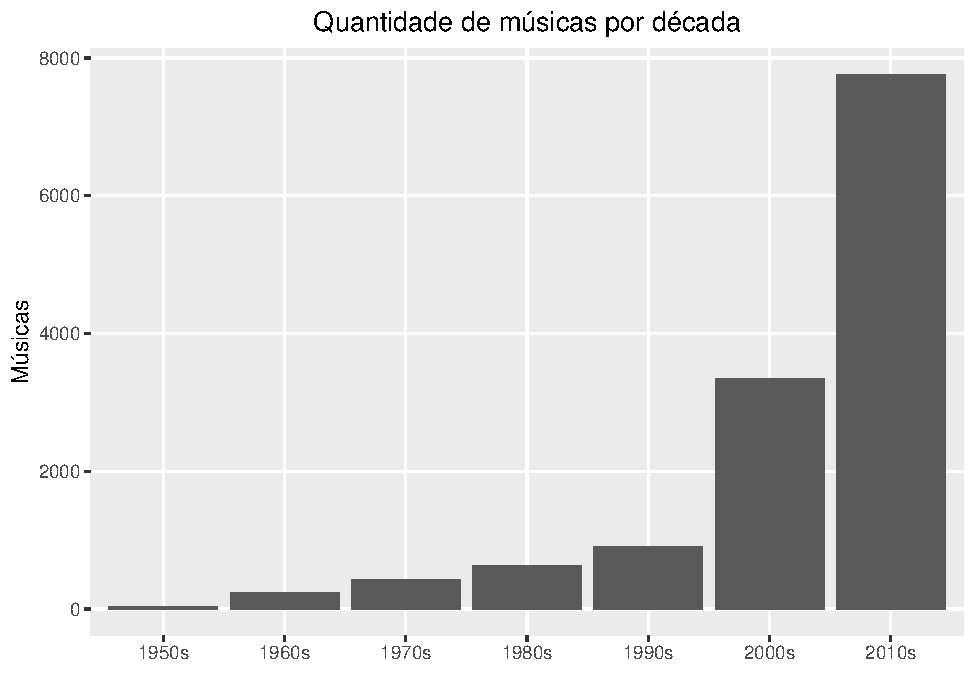
\includegraphics{avaliacaoLetrasDeForro_files/figure-latex/unnamed-chunk-4-1.pdf}

\hypertarget{quantidade-de-palavras-utilizadas-por-decada}{%
\section{Quantidade de palavras utilizadas por
década}\label{quantidade-de-palavras-utilizadas-por-decada}}

Em uma análise inicial mais rasa podemos visualizar a quantidade geral
de palavras utilizadas por década. Apesar de ser uma análise simples, ja
podemos observar algumas palavras que continuam sendo utilizadas, apesar
dos anos.

\begin{Shaded}
\begin{Highlighting}[]
\NormalTok{musicas_filtradas <-}\StringTok{ }\NormalTok{musicas }\OperatorTok
\StringTok{  }\KeywordTok{unnest_tokens}\NormalTok{(word, letra) }\OperatorTok
\StringTok{  }\KeywordTok{anti_join}\NormalTok{(stopwords_pt) }\OperatorTok
\StringTok{  }\KeywordTok{distinct}\NormalTok{() }\OperatorTok
\StringTok{  }\KeywordTok{filter}\NormalTok{(}\OperatorTok{!}\NormalTok{word }\OperatorTok\StringTok{ }\NormalTok{palavras_indesejadas) }\OperatorTok
\StringTok{  }\KeywordTok{filter}\NormalTok{(}\KeywordTok{nchar}\NormalTok{(word) }\OperatorTok{>}\StringTok{ }\DecValTok{3}\NormalTok{)}


\NormalTok{ContaPalavrasUtilizadasPorDecada <-}\StringTok{ }\ControlFlowTok{function}\NormalTok{(d) \{}
\NormalTok{  ds <-}\StringTok{ }\NormalTok{musicas_filtradas }\OperatorTok\StringTok{ }\KeywordTok{filter}\NormalTok{(decada }\OperatorTok{==}\StringTok{ }\NormalTok{d)}
  
\NormalTok{  ds }\OperatorTok
\StringTok{  }\KeywordTok{count}\NormalTok{(word, }\DataTypeTok{sort =} \OtherTok{TRUE}\NormalTok{) }\OperatorTok
\StringTok{  }\KeywordTok{top_n}\NormalTok{(}\DecValTok{10}\NormalTok{) }\OperatorTok
\StringTok{  }\KeywordTok{ungroup}\NormalTok{() }\OperatorTok
\StringTok{  }\KeywordTok{mutate}\NormalTok{(}\DataTypeTok{word =} \KeywordTok{reorder}\NormalTok{(word, n)) }\OperatorTok
\StringTok{  }\KeywordTok{ggplot}\NormalTok{() }\OperatorTok{+}
\StringTok{    }\KeywordTok{geom_col}\NormalTok{(}\KeywordTok{aes}\NormalTok{(word, n), }\DataTypeTok{fill =}\NormalTok{ colors[}\DecValTok{4}\NormalTok{]) }\OperatorTok{+}
\StringTok{    }\KeywordTok{theme}\NormalTok{(}\DataTypeTok{legend.position =} \StringTok{"none"}\NormalTok{, }
          \DataTypeTok{plot.title =} \KeywordTok{element_text}\NormalTok{(}\DataTypeTok{hjust =} \FloatTok{0.5}\NormalTok{),}
          \DataTypeTok{panel.grid.major =} \KeywordTok{element_blank}\NormalTok{()) }\OperatorTok{+}
\StringTok{    }\KeywordTok{xlab}\NormalTok{(}\StringTok{""}\NormalTok{) }\OperatorTok{+}\StringTok{ }
\StringTok{    }\KeywordTok{ylab}\NormalTok{(}\StringTok{"Quantidade de músicas") +}
\StringTok{    ggtitle("}\NormalTok{Palavras}\StringTok{") +}
\StringTok{    coord_flip()}
\StringTok{\}}

\StringTok{ContaPalavrasUtilizadasPorDecada("}\NormalTok{1950s}\StringTok{")}
\end{Highlighting}
\end{Shaded}

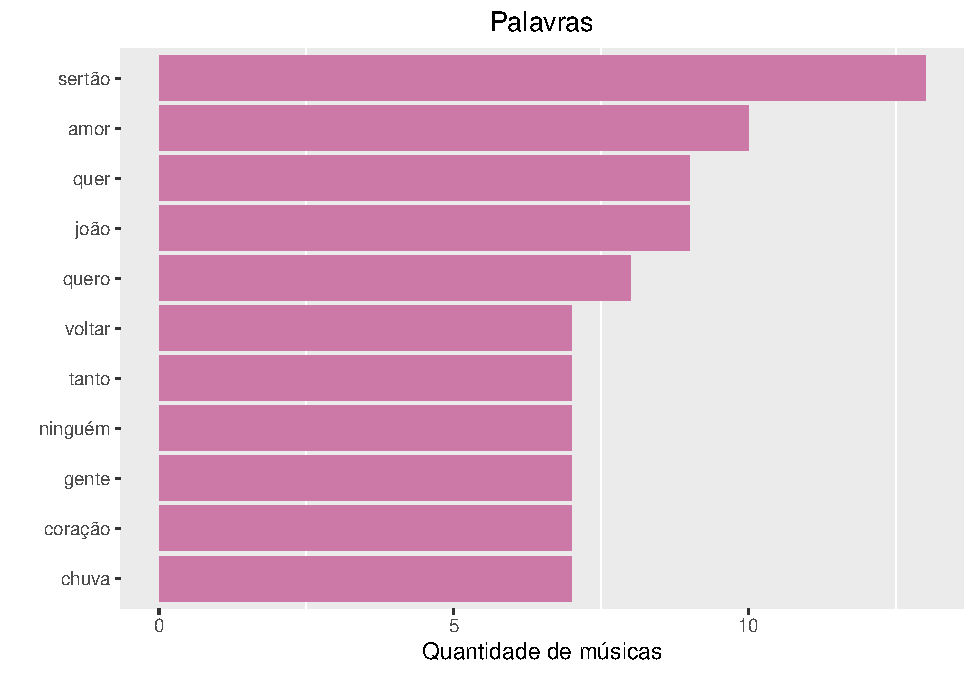
\includegraphics{avaliacaoLetrasDeForro_files/figure-latex/unnamed-chunk-5-1.pdf}

\begin{Shaded}
\begin{Highlighting}[]
\KeywordTok{ContaPalavrasUtilizadasPorDecada}\NormalTok{(}\StringTok{"1960s"}\NormalTok{)}
\end{Highlighting}
\end{Shaded}

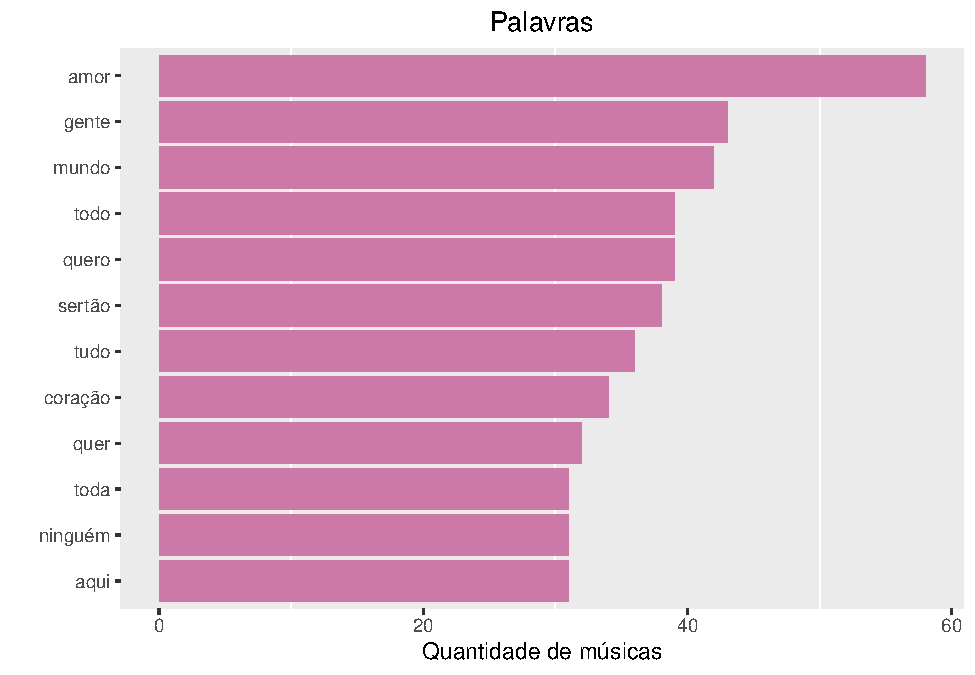
\includegraphics{avaliacaoLetrasDeForro_files/figure-latex/unnamed-chunk-5-2.pdf}

\begin{Shaded}
\begin{Highlighting}[]
\KeywordTok{ContaPalavrasUtilizadasPorDecada}\NormalTok{(}\StringTok{"1970s"}\NormalTok{)}
\end{Highlighting}
\end{Shaded}

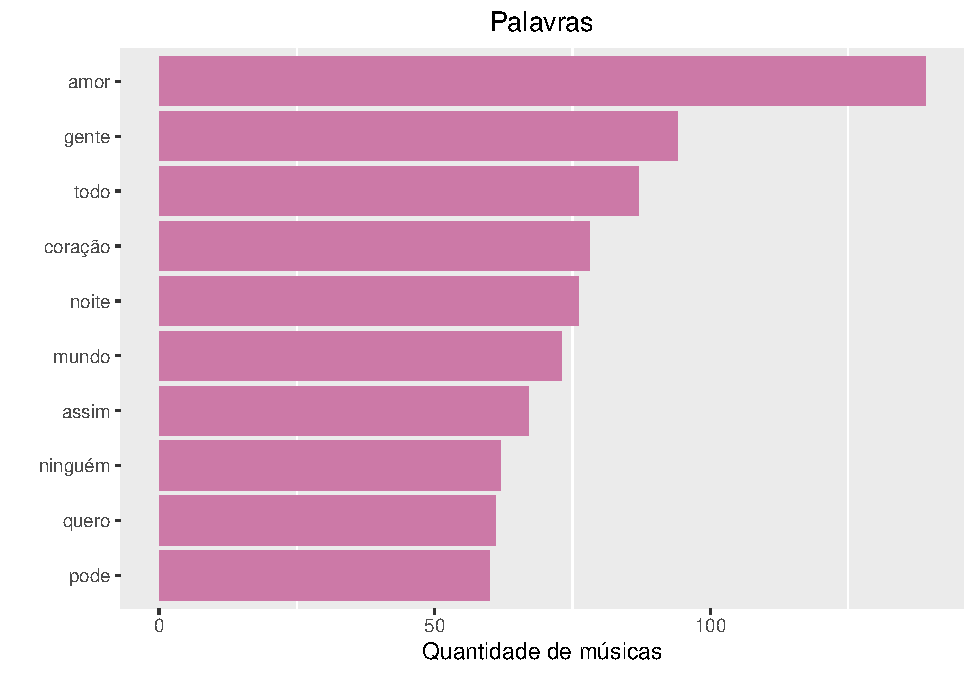
\includegraphics{avaliacaoLetrasDeForro_files/figure-latex/unnamed-chunk-5-3.pdf}

\begin{Shaded}
\begin{Highlighting}[]
\KeywordTok{ContaPalavrasUtilizadasPorDecada}\NormalTok{(}\StringTok{"1980s"}\NormalTok{)}
\end{Highlighting}
\end{Shaded}

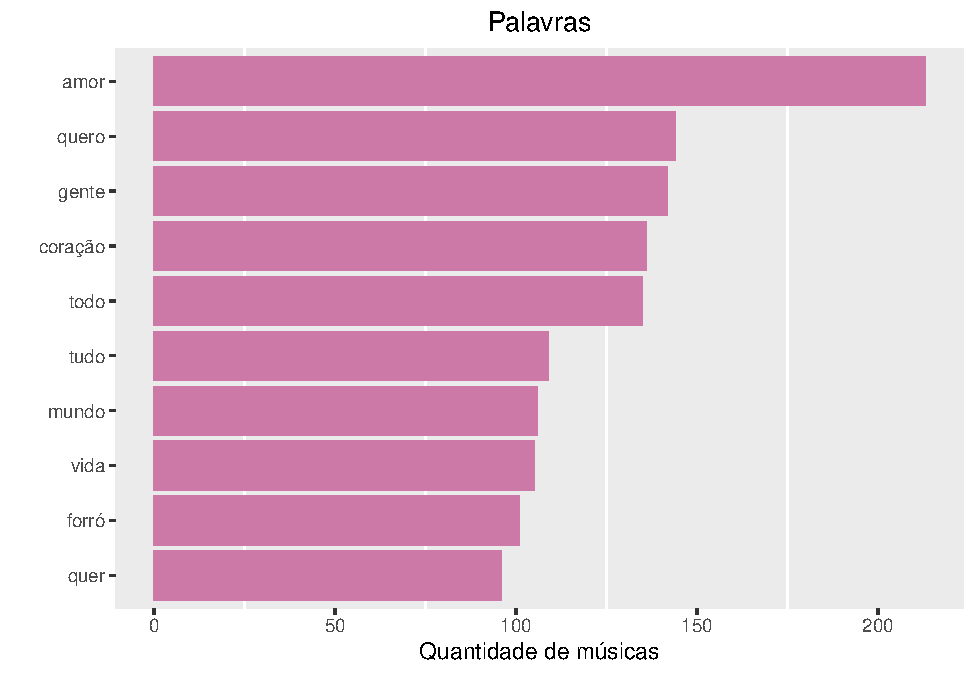
\includegraphics{avaliacaoLetrasDeForro_files/figure-latex/unnamed-chunk-5-4.pdf}

\begin{Shaded}
\begin{Highlighting}[]
\KeywordTok{ContaPalavrasUtilizadasPorDecada}\NormalTok{(}\StringTok{"1990s"}\NormalTok{)}
\end{Highlighting}
\end{Shaded}

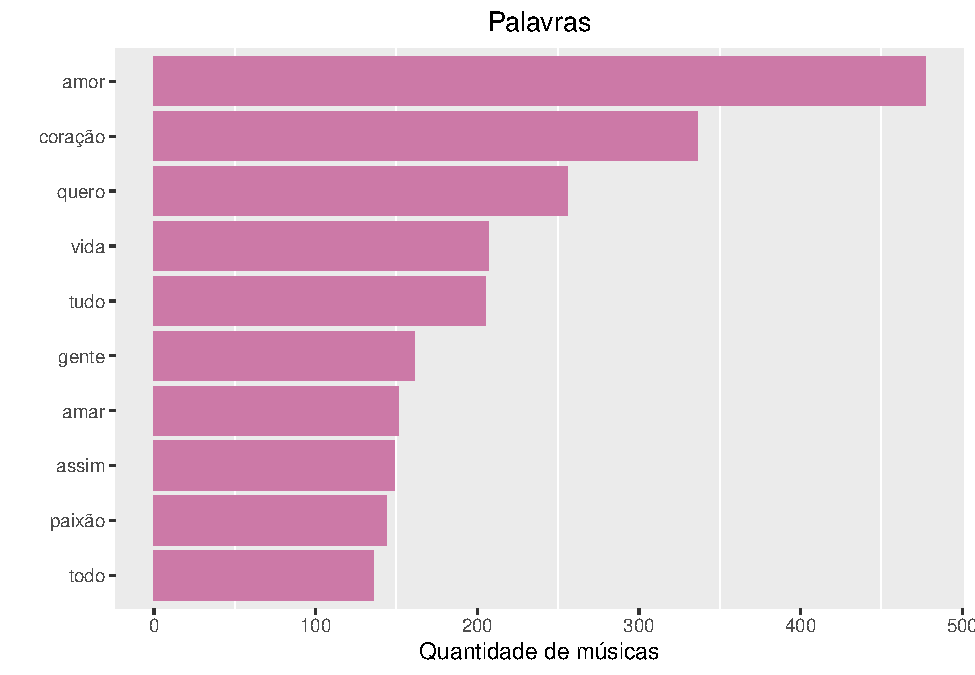
\includegraphics{avaliacaoLetrasDeForro_files/figure-latex/unnamed-chunk-5-5.pdf}

\begin{Shaded}
\begin{Highlighting}[]
\KeywordTok{ContaPalavrasUtilizadasPorDecada}\NormalTok{(}\StringTok{"2000s"}\NormalTok{)}
\end{Highlighting}
\end{Shaded}

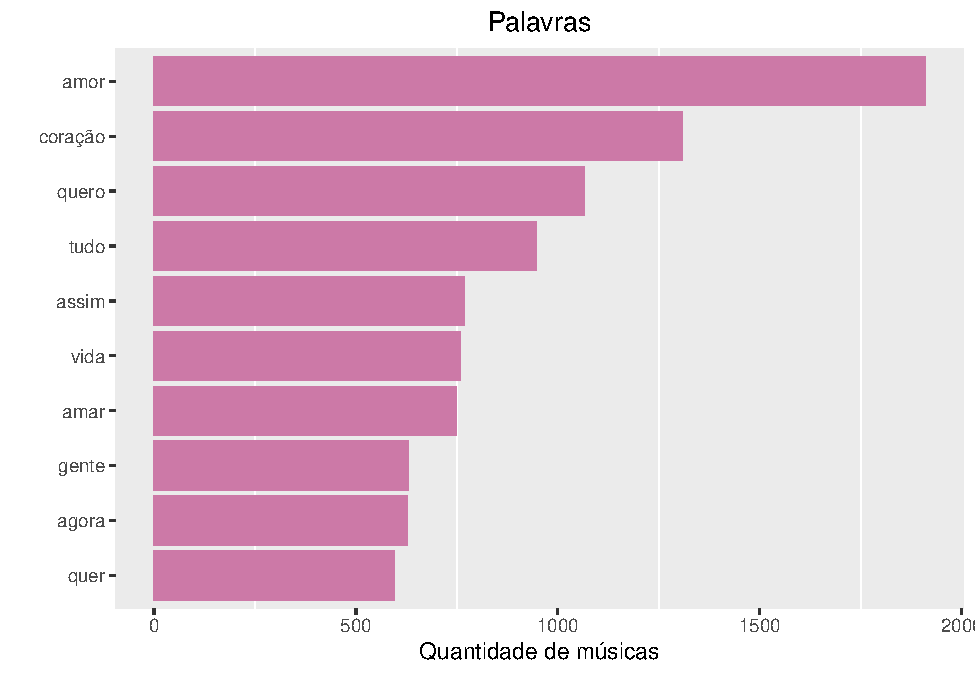
\includegraphics{avaliacaoLetrasDeForro_files/figure-latex/unnamed-chunk-5-6.pdf}

\begin{Shaded}
\begin{Highlighting}[]
\KeywordTok{ContaPalavrasUtilizadasPorDecada}\NormalTok{(}\StringTok{"2010s"}\NormalTok{)}
\end{Highlighting}
\end{Shaded}

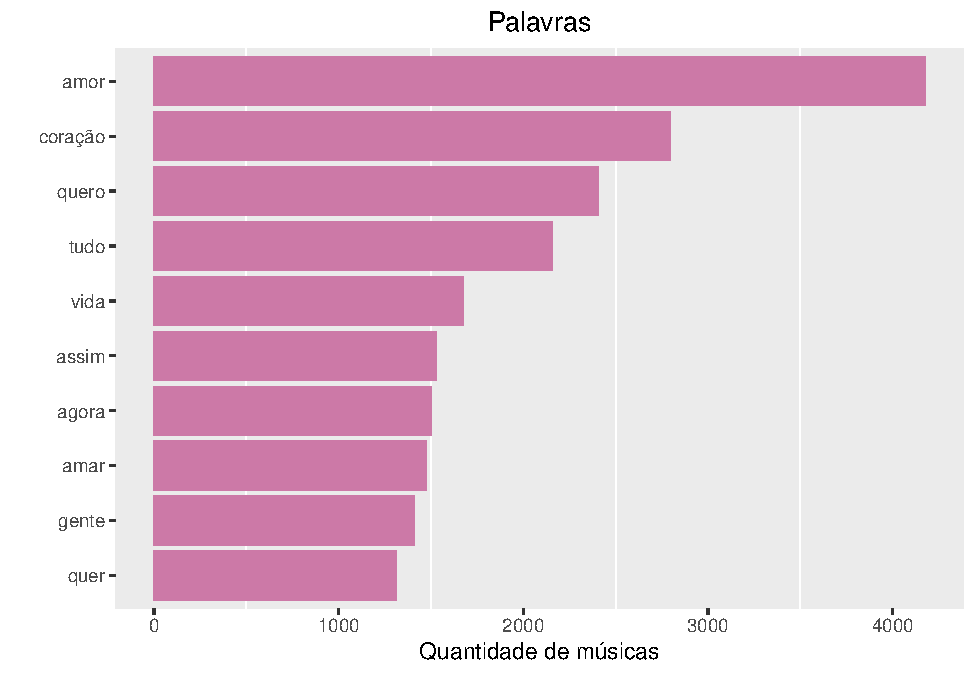
\includegraphics{avaliacaoLetrasDeForro_files/figure-latex/unnamed-chunk-5-7.pdf}

\hypertarget{nuvens-de-palavras-em-relacao-a-quantidade-de-palavras-utilizadas-por-decada}{%
\section{Núvens de palavras em relação a quantidade de palavras
utilizadas por
década}\label{nuvens-de-palavras-em-relacao-a-quantidade-de-palavras-utilizadas-por-decada}}

\begin{Shaded}
\begin{Highlighting}[]
\NormalTok{quantidade_palavras <-}\StringTok{ }\NormalTok{musicas_filtradas }\OperatorTok
\StringTok{  }\KeywordTok{count}\NormalTok{(word, }\DataTypeTok{sort =} \OtherTok{TRUE}\NormalTok{)}

\NormalTok{ContaPalavras<-}\StringTok{ }\ControlFlowTok{function}\NormalTok{(ds_filtered) \{}
\NormalTok{  result <-}\StringTok{ }\NormalTok{ds_filtered }\OperatorTok\StringTok{ }\KeywordTok{count}\NormalTok{(word, }\DataTypeTok{sort =} \OtherTok{TRUE}\NormalTok{)}
  \KeywordTok{return}\NormalTok{(result)}
\NormalTok{\}}

\NormalTok{filtraMusicasPorDecada <-}\StringTok{ }\ControlFlowTok{function}\NormalTok{(d) \{}
\NormalTok{  ds_filtered <-}\StringTok{ }\NormalTok{musicas }\OperatorTok\StringTok{ }\KeywordTok{filter}\NormalTok{(decada }\OperatorTok{==}\StringTok{ }\NormalTok{d)}
  
\NormalTok{  result <-}\StringTok{ }\NormalTok{ds_filtered }\OperatorTok
\StringTok{  }\KeywordTok{unnest_tokens}\NormalTok{(word, letra) }\OperatorTok
\StringTok{  }\KeywordTok{anti_join}\NormalTok{(stopwords_pt, }\DataTypeTok{by=}\StringTok{"word"}\NormalTok{) }\OperatorTok
\StringTok{  }\KeywordTok{distinct}\NormalTok{() }\OperatorTok
\StringTok{  }\KeywordTok{filter}\NormalTok{(}\OperatorTok{!}\NormalTok{word }\OperatorTok\StringTok{ }\NormalTok{palavras_indesejadas) }\OperatorTok
\StringTok{  }\KeywordTok{filter}\NormalTok{(}\KeywordTok{nchar}\NormalTok{(word) }\OperatorTok{>}\StringTok{ }\DecValTok{3}\NormalTok{)}
  \KeywordTok{return}\NormalTok{(result)}
\NormalTok{\}}


\KeywordTok{wordcloud2}\NormalTok{((}\KeywordTok{filtraMusicasPorDecada}\NormalTok{(}\StringTok{"1950s"}\NormalTok{) }\OperatorTok\StringTok{  }\NormalTok{ContaPalavras)[}\DecValTok{1}\OperatorTok{:}\DecValTok{100}\NormalTok{, ], }\DataTypeTok{size =} \FloatTok{.4}\NormalTok{, }\KeywordTok{options}\NormalTok{(}\DataTypeTok{warn =} \DecValTok{0}\NormalTok{))}
\end{Highlighting}
\end{Shaded}

\includegraphics{avaliacaoLetrasDeForro_files/figure-latex/unnamed-chunk-6-1.pdf}

\begin{Shaded}
\begin{Highlighting}[]
\KeywordTok{wordcloud2}\NormalTok{((}\KeywordTok{filtraMusicasPorDecada}\NormalTok{(}\StringTok{"1960s"}\NormalTok{) }\OperatorTok\StringTok{  }\NormalTok{ContaPalavras)[}\DecValTok{1}\OperatorTok{:}\DecValTok{100}\NormalTok{, ], }\DataTypeTok{size =} \FloatTok{.4}\NormalTok{, }\KeywordTok{options}\NormalTok{(}\DataTypeTok{warn =} \DecValTok{0}\NormalTok{))}
\end{Highlighting}
\end{Shaded}

\includegraphics{avaliacaoLetrasDeForro_files/figure-latex/unnamed-chunk-6-2.pdf}

\begin{Shaded}
\begin{Highlighting}[]
\KeywordTok{wordcloud2}\NormalTok{((}\KeywordTok{filtraMusicasPorDecada}\NormalTok{(}\StringTok{"1970s"}\NormalTok{) }\OperatorTok\StringTok{  }\NormalTok{ContaPalavras)[}\DecValTok{1}\OperatorTok{:}\DecValTok{100}\NormalTok{, ], }\DataTypeTok{size =} \FloatTok{.4}\NormalTok{, }\KeywordTok{options}\NormalTok{(}\DataTypeTok{warn =} \DecValTok{0}\NormalTok{))}
\end{Highlighting}
\end{Shaded}

\includegraphics{avaliacaoLetrasDeForro_files/figure-latex/unnamed-chunk-6-3.pdf}

\begin{Shaded}
\begin{Highlighting}[]
\KeywordTok{wordcloud2}\NormalTok{((}\KeywordTok{filtraMusicasPorDecada}\NormalTok{(}\StringTok{"1980s"}\NormalTok{) }\OperatorTok\StringTok{  }\NormalTok{ContaPalavras)[}\DecValTok{1}\OperatorTok{:}\DecValTok{100}\NormalTok{, ], }\DataTypeTok{size =} \FloatTok{.4}\NormalTok{, }\KeywordTok{options}\NormalTok{(}\DataTypeTok{warn =} \DecValTok{0}\NormalTok{))}
\end{Highlighting}
\end{Shaded}

\includegraphics{avaliacaoLetrasDeForro_files/figure-latex/unnamed-chunk-6-4.pdf}

\begin{Shaded}
\begin{Highlighting}[]
\KeywordTok{wordcloud2}\NormalTok{((}\KeywordTok{filtraMusicasPorDecada}\NormalTok{(}\StringTok{"1990s"}\NormalTok{) }\OperatorTok\StringTok{  }\NormalTok{ContaPalavras)[}\DecValTok{1}\OperatorTok{:}\DecValTok{100}\NormalTok{, ], }\DataTypeTok{size =} \FloatTok{.4}\NormalTok{, }\KeywordTok{options}\NormalTok{(}\DataTypeTok{warn =} \DecValTok{0}\NormalTok{))}
\end{Highlighting}
\end{Shaded}

\includegraphics{avaliacaoLetrasDeForro_files/figure-latex/unnamed-chunk-6-5.pdf}

\begin{Shaded}
\begin{Highlighting}[]
\KeywordTok{wordcloud2}\NormalTok{((}\KeywordTok{filtraMusicasPorDecada}\NormalTok{(}\StringTok{"2000s"}\NormalTok{) }\OperatorTok\StringTok{  }\NormalTok{ContaPalavras)[}\DecValTok{1}\OperatorTok{:}\DecValTok{100}\NormalTok{, ], }\DataTypeTok{size =} \FloatTok{.4}\NormalTok{, }\KeywordTok{options}\NormalTok{(}\DataTypeTok{warn =} \DecValTok{0}\NormalTok{))}
\end{Highlighting}
\end{Shaded}

\includegraphics{avaliacaoLetrasDeForro_files/figure-latex/unnamed-chunk-6-6.pdf}

\begin{Shaded}
\begin{Highlighting}[]
\KeywordTok{wordcloud2}\NormalTok{((}\KeywordTok{filtraMusicasPorDecada}\NormalTok{(}\StringTok{"2010s"}\NormalTok{) }\OperatorTok\StringTok{  }\NormalTok{ContaPalavras)[}\DecValTok{1}\OperatorTok{:}\DecValTok{100}\NormalTok{, ], }\DataTypeTok{size =} \FloatTok{.4}\NormalTok{, }\KeywordTok{options}\NormalTok{(}\DataTypeTok{warn =} \DecValTok{0}\NormalTok{))}
\end{Highlighting}
\end{Shaded}

\includegraphics{avaliacaoLetrasDeForro_files/figure-latex/unnamed-chunk-6-7.pdf}

\hypertarget{palavras-atemporais}{%
\section{Palavras Atemporais}\label{palavras-atemporais}}

Podemos visualizar nos gráficos a seguir, quais são as palavras que
continuam sendo utilizadas independente do decorrer do tempo.

As palavras de interesse, sobem para o topo de cada gráfico. Em geral
podemos perceber a permanencia de palavras como: ``amor'', ``coração'',
``gente'' etc.

\begin{Shaded}
\begin{Highlighting}[]
\NormalTok{palavras_atemporais <-}\StringTok{ }\NormalTok{musicas_filtradas }\OperatorTok\StringTok{ }
\StringTok{  }\KeywordTok{filter}\NormalTok{(decada }\OperatorTok{!=}\StringTok{ 'NA'}\NormalTok{) }\OperatorTok
\StringTok{  }\KeywordTok{group_by}\NormalTok{(decada) }\OperatorTok
\StringTok{  }\KeywordTok{count}\NormalTok{(word, decada, }\DataTypeTok{sort =} \OtherTok{TRUE}\NormalTok{) }\OperatorTok
\StringTok{  }\KeywordTok{slice}\NormalTok{(}\KeywordTok{seq_len}\NormalTok{(}\DecValTok{8}\NormalTok{)) }\OperatorTok
\StringTok{  }\KeywordTok{ungroup}\NormalTok{() }\OperatorTok
\StringTok{  }\KeywordTok{arrange}\NormalTok{(decada,n) }\OperatorTok
\StringTok{  }\KeywordTok{mutate}\NormalTok{(}\DataTypeTok{row =} \KeywordTok{row_number}\NormalTok{()) }

\NormalTok{palavras_atemporais }\OperatorTok
\StringTok{  }\KeywordTok{ggplot}\NormalTok{(}\KeywordTok{aes}\NormalTok{(row, n, }\DataTypeTok{fill =}\NormalTok{ decada)) }\OperatorTok{+}
\StringTok{    }\KeywordTok{geom_col}\NormalTok{(}\DataTypeTok{show.legend =} \OtherTok{NULL}\NormalTok{) }\OperatorTok{+}
\StringTok{    }\KeywordTok{labs}\NormalTok{(}\DataTypeTok{x =} \OtherTok{NULL}\NormalTok{, }\DataTypeTok{y =} \StringTok{"Palavras"}\NormalTok{) }\OperatorTok{+}
\StringTok{    }\KeywordTok{ggtitle}\NormalTok{(}\StringTok{"Palavras Atemporaris"}\NormalTok{) }\OperatorTok{+}\StringTok{ }
\StringTok{    }\KeywordTok{theme_lyrics}\NormalTok{() }\OperatorTok{+}\StringTok{  }
\StringTok{    }\KeywordTok{facet_wrap}\NormalTok{(}\OperatorTok{~}\NormalTok{decada, }\DataTypeTok{scales =} \StringTok{"free"}\NormalTok{, }\DataTypeTok{ncol =} \DecValTok{5}\NormalTok{) }\OperatorTok{+}
\StringTok{    }\KeywordTok{scale_x_continuous}\NormalTok{(}\DataTypeTok{breaks =}\NormalTok{ palavras_atemporais}\OperatorTok{$}\NormalTok{row, }\DataTypeTok{labels =}\NormalTok{ palavras_atemporais}\OperatorTok{$}\NormalTok{word) }\OperatorTok{+}
\StringTok{    }\KeywordTok{coord_flip}\NormalTok{()}
\end{Highlighting}
\end{Shaded}

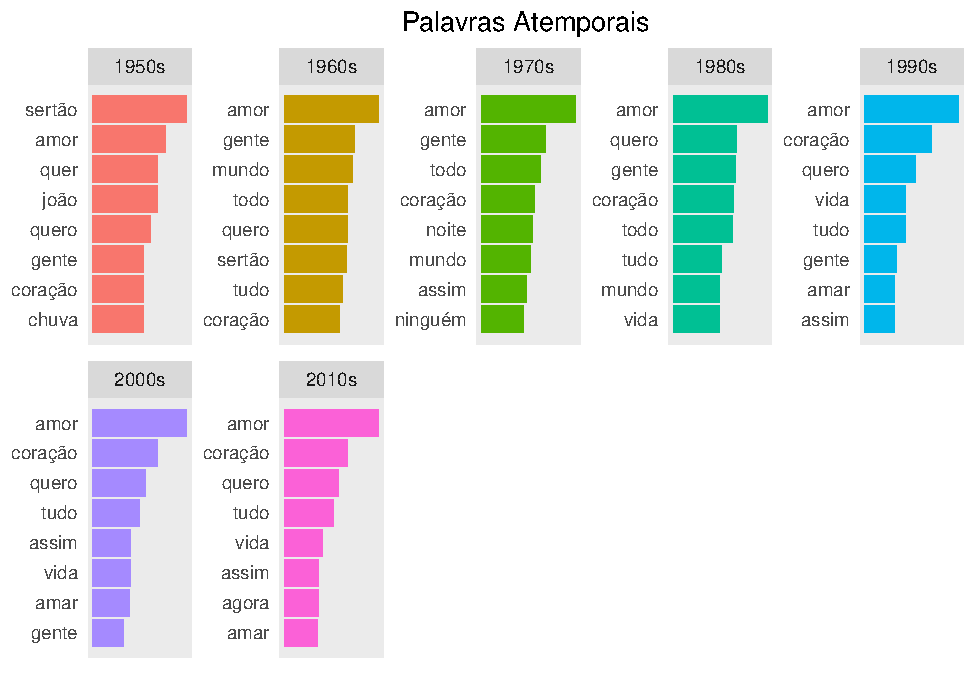
\includegraphics{avaliacaoLetrasDeForro_files/figure-latex/unnamed-chunk-7-1.pdf}

\hypertarget{relacao-sobre-o-tamanho-das-palavras-e-o-tamanho-das-letras-ao-longo-do-tempo}{%
\section{Relação sobre o tamanho das palavras e o tamanho das letras ao
longo do
tempo}\label{relacao-sobre-o-tamanho-das-palavras-e-o-tamanho-das-letras-ao-longo-do-tempo}}

Palavras maiores podem acrescentar complexidade nas letras e também
podem indicar se as letras podem ser mais ou menos complexas.

O ponto de observação principal aqui é a relação entre quantidade de
palavras por música e o tamanho das palavras. Podemos observar que são
dois pontos inversamente proporcionais onde, quanto mais palavras a
letra possui, menor o tamanho das palavras.

()

\begin{Shaded}
\begin{Highlighting}[]
\NormalTok{ContaTamangoDasPalavrasPorDecada <-}\StringTok{ }\ControlFlowTok{function}\NormalTok{(d) \{}
\NormalTok{  ds <-}\StringTok{ }\NormalTok{musicas }\OperatorTok\StringTok{ }\KeywordTok{filter}\NormalTok{(decada }\OperatorTok{==}\StringTok{ }\NormalTok{d)}
\NormalTok{  result <-}\StringTok{ }\NormalTok{ds }\OperatorTok
\StringTok{  }\KeywordTok{unnest_tokens}\NormalTok{(word, letra) }\OperatorTok
\StringTok{  }\KeywordTok{group_by}\NormalTok{(nome, decada) }\OperatorTok
\StringTok{  }\KeywordTok{distinct}\NormalTok{() }\OperatorTok
\StringTok{  }\KeywordTok{filter}\NormalTok{(}\OperatorTok{!}\NormalTok{word }\OperatorTok\StringTok{ }\NormalTok{palavras_indesejadas) }\OperatorTok
\StringTok{  }\KeywordTok{mutate}\NormalTok{(}\DataTypeTok{word_length =} \KeywordTok{nchar}\NormalTok{(word))}
  \KeywordTok{return}\NormalTok{(result)}
\NormalTok{\}}

\NormalTok{PlotaTamanhosDasPalavras <-}\StringTok{ }\ControlFlowTok{function}\NormalTok{(word_lengths, decada) \{}
\NormalTok{  word_lengths }\OperatorTok
\StringTok{  }\KeywordTok{count}\NormalTok{(word_length, }\DataTypeTok{sort =} \OtherTok{TRUE}\NormalTok{) }\OperatorTok
\StringTok{  }\KeywordTok{ggplot}\NormalTok{(}\KeywordTok{aes}\NormalTok{(word_length), }\DataTypeTok{binwidth =} \DecValTok{10}\NormalTok{) }\OperatorTok{+}\StringTok{ }
\StringTok{  }\KeywordTok{geom_histogram}\NormalTok{(}\KeywordTok{aes}\NormalTok{(}\DataTypeTok{fill =}\NormalTok{ ..count..), }\DataTypeTok{breaks =} \KeywordTok{seq}\NormalTok{(}\DecValTok{1}\NormalTok{,}\DecValTok{25}\NormalTok{, }\DataTypeTok{by =} \DecValTok{2}\NormalTok{),}
  \DataTypeTok{show.legend =} \OtherTok{FALSE}\NormalTok{) }\OperatorTok{+}\StringTok{ }
\StringTok{  }\KeywordTok{xlab}\NormalTok{(}\StringTok{"Tamanho das palavras"}\NormalTok{) }\OperatorTok{+}\StringTok{ }\KeywordTok{ylab}\NormalTok{(}\StringTok{"Quantidade das palavras"}\NormalTok{) }\OperatorTok{+}
\StringTok{  }\KeywordTok{ggtitle}\NormalTok{(}\KeywordTok{paste}\NormalTok{(}\StringTok{"Distribuição do tamanho das palavras a década de "}\NormalTok{)) }\OperatorTok{+}
\StringTok{  }\KeywordTok{theme}\NormalTok{(}\DataTypeTok{plot.title =} \KeywordTok{element_text}\NormalTok{(}\DataTypeTok{hjust =} \FloatTok{0.5}\NormalTok{), }\DataTypeTok{panel.grid.minor =} \KeywordTok{element_blank}\NormalTok{())}
\NormalTok{\}}

\KeywordTok{PlotaTamanhosDasPalavras}\NormalTok{(}\KeywordTok{ContaTamangoDasPalavrasPorDecada}\NormalTok{(}\StringTok{"1950s"}\NormalTok{), }\StringTok{"1950s"}\NormalTok{)}
\end{Highlighting}
\end{Shaded}

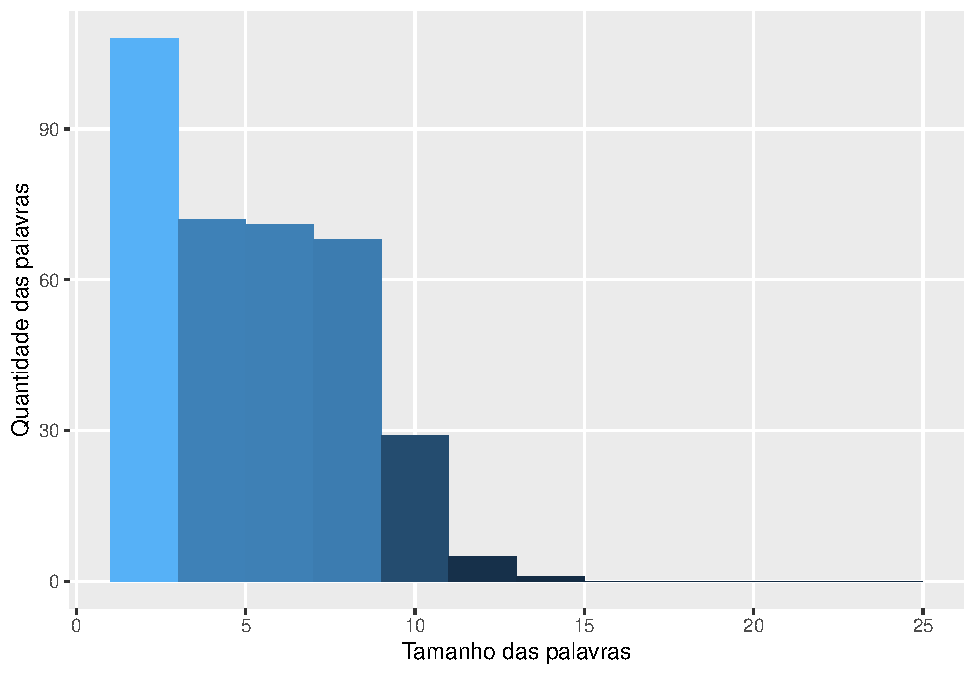
\includegraphics{avaliacaoLetrasDeForro_files/figure-latex/unnamed-chunk-8-1.pdf}

\begin{Shaded}
\begin{Highlighting}[]
\KeywordTok{PlotaTamanhosDasPalavras}\NormalTok{(}\KeywordTok{ContaTamangoDasPalavrasPorDecada}\NormalTok{(}\StringTok{"1960s"}\NormalTok{), }\StringTok{"1960s"}\NormalTok{)}
\end{Highlighting}
\end{Shaded}

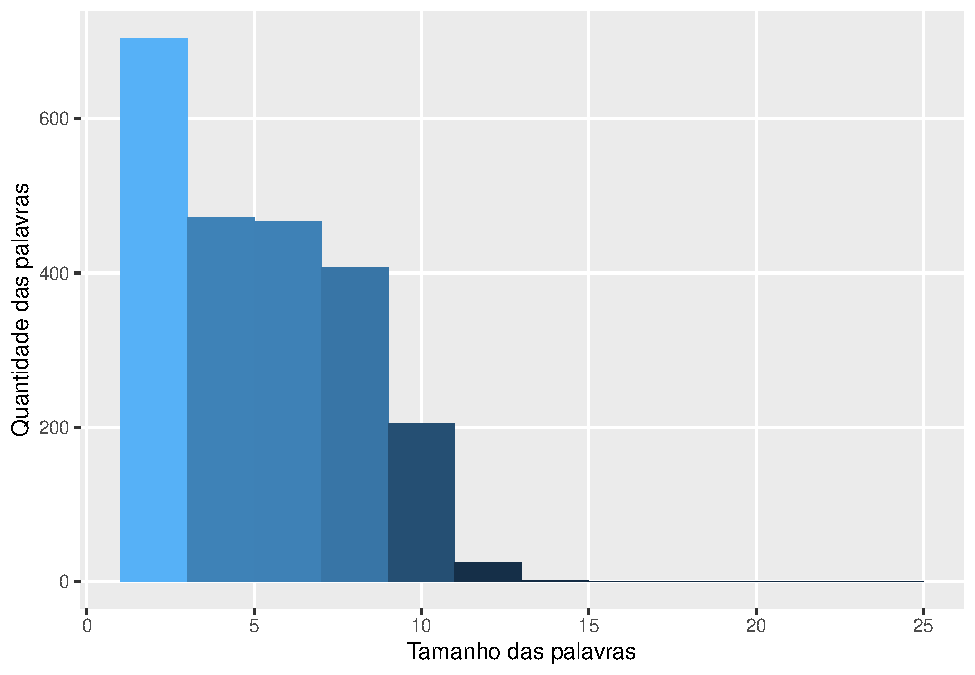
\includegraphics{avaliacaoLetrasDeForro_files/figure-latex/unnamed-chunk-8-2.pdf}

\begin{Shaded}
\begin{Highlighting}[]
\KeywordTok{PlotaTamanhosDasPalavras}\NormalTok{(}\KeywordTok{ContaTamangoDasPalavrasPorDecada}\NormalTok{(}\StringTok{"1970s"}\NormalTok{), }\StringTok{"1970s"}\NormalTok{)}
\end{Highlighting}
\end{Shaded}

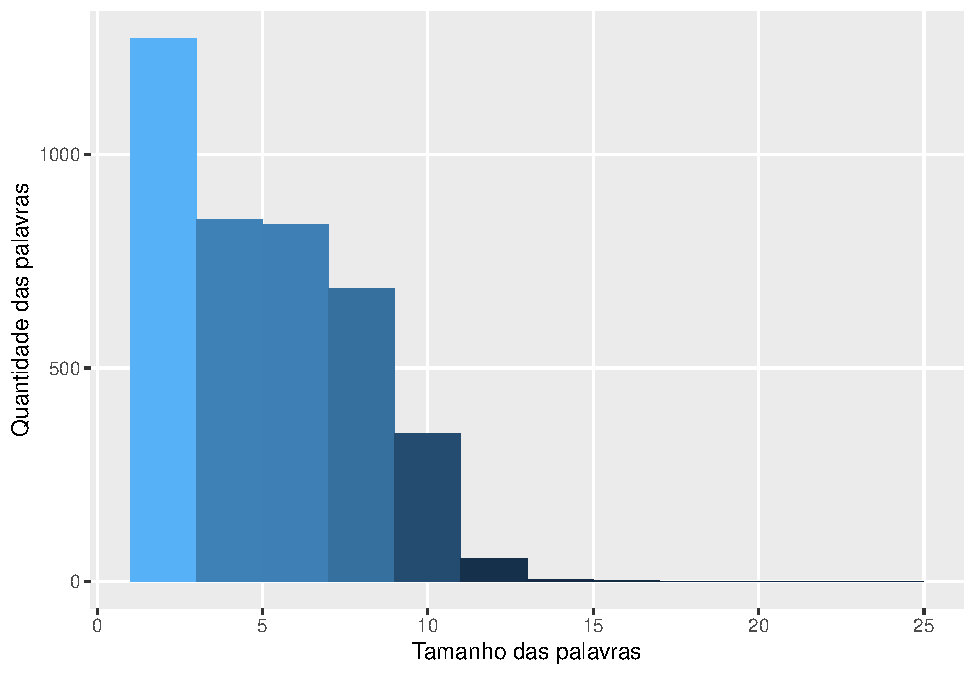
\includegraphics{avaliacaoLetrasDeForro_files/figure-latex/unnamed-chunk-8-3.pdf}

\begin{Shaded}
\begin{Highlighting}[]
\KeywordTok{PlotaTamanhosDasPalavras}\NormalTok{(}\KeywordTok{ContaTamangoDasPalavrasPorDecada}\NormalTok{(}\StringTok{"1980s"}\NormalTok{), }\StringTok{"1980s"}\NormalTok{)}
\end{Highlighting}
\end{Shaded}

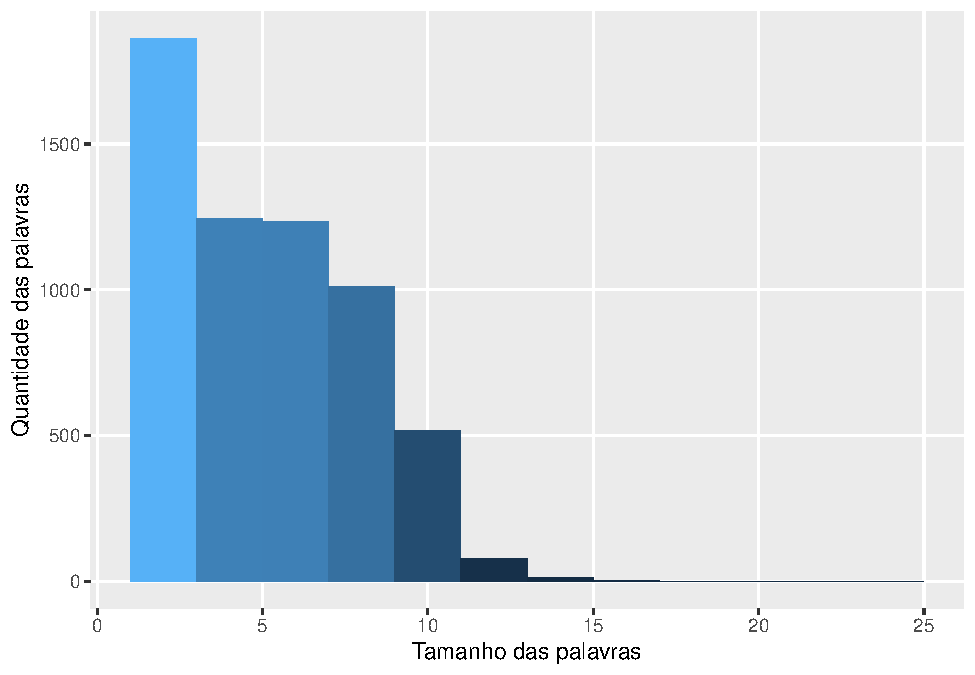
\includegraphics{avaliacaoLetrasDeForro_files/figure-latex/unnamed-chunk-8-4.pdf}

\begin{Shaded}
\begin{Highlighting}[]
\KeywordTok{PlotaTamanhosDasPalavras}\NormalTok{(}\KeywordTok{ContaTamangoDasPalavrasPorDecada}\NormalTok{(}\StringTok{"1990s"}\NormalTok{), }\StringTok{"1990s"}\NormalTok{)}
\end{Highlighting}
\end{Shaded}

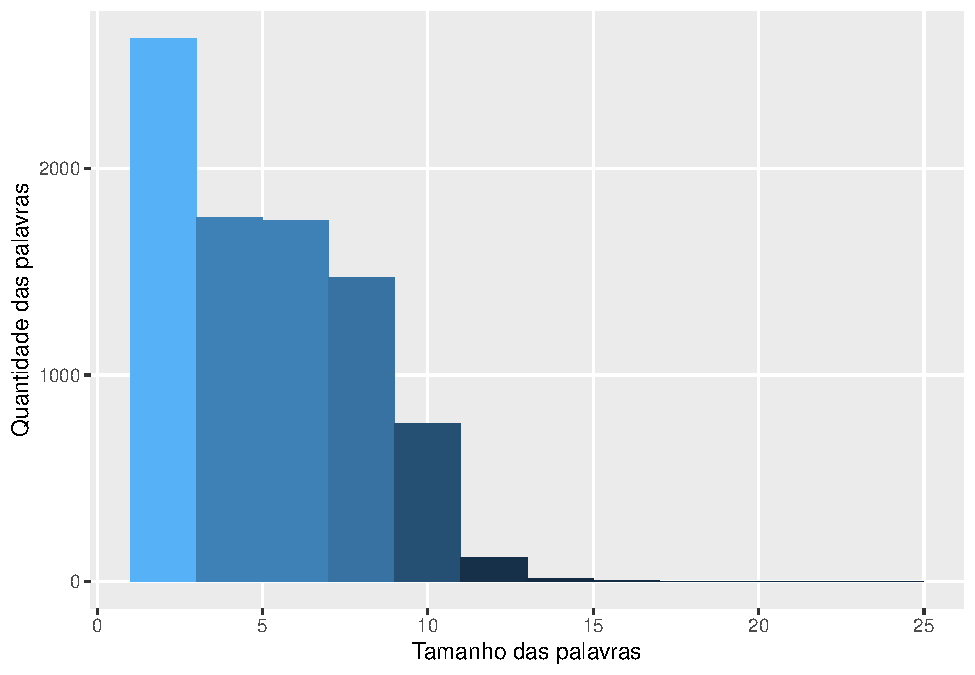
\includegraphics{avaliacaoLetrasDeForro_files/figure-latex/unnamed-chunk-8-5.pdf}

\begin{Shaded}
\begin{Highlighting}[]
\KeywordTok{PlotaTamanhosDasPalavras}\NormalTok{(}\KeywordTok{ContaTamangoDasPalavrasPorDecada}\NormalTok{(}\StringTok{"2000s"}\NormalTok{), }\StringTok{"2000s"}\NormalTok{)}
\end{Highlighting}
\end{Shaded}

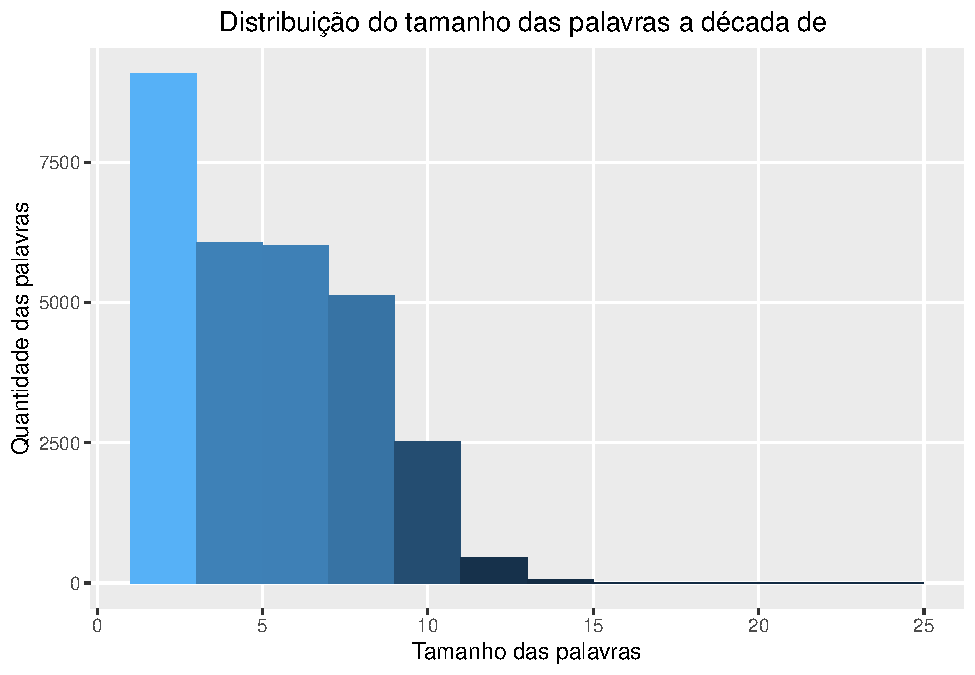
\includegraphics{avaliacaoLetrasDeForro_files/figure-latex/unnamed-chunk-8-6.pdf}

\hypertarget{densidade-e-diversidade-lexical-distribuicao-e-diversidade-do-vocabulario}{%
\section{Densidade e Diversidade Lexical / Distribuição e Diversidade do
vocabulário}\label{densidade-e-diversidade-lexical-distribuicao-e-diversidade-do-vocabulario}}

Podemos observar o gráfico de distribuição das palavras no decorrer do
tempo, para visualizar como as palavras exclusivas se distribuem no
decorrer do tempo e avaliar a tendência das composições em relação a
repetição de palavras no decorrer do tempo.

Sabendo que a quantidade de letras passou por um crescimento acentuado
no decorrer tempo, o gráfico indica um leve decaimento da densidade de
palavras exclusivas no decorrer do tempo. Mesmo que seja uma avaliação
subjetiva, podemos crer que, com o passar do tempo, mais as letras
repetiram palavras e ficaram mais ``pobres'' em termos de seu
vocabulário e também que as letras são mais repetitivas.

Na diversidade de palavras, o gráfico demonstra a média de palavras
únicas ao longo do tempo. Reforça a avaliação baseada na densidade e nos
indica como as palavras únicas evoluíram ao longo do tempo em termos de
quantidade.

\begin{Shaded}
\begin{Highlighting}[]
\NormalTok{densidade_lexical_por_ano <-}\StringTok{ }\NormalTok{musicas }\OperatorTok
\StringTok{  }\KeywordTok{filter}\NormalTok{(decada }\OperatorTok{!=}\StringTok{ "NA"}\NormalTok{) }\OperatorTok
\StringTok{  }\KeywordTok{unnest_tokens}\NormalTok{(word, letra) }\OperatorTok
\StringTok{  }\KeywordTok{group_by}\NormalTok{(nome,ano) }\OperatorTok
\StringTok{  }\KeywordTok{summarise}\NormalTok{(}\DataTypeTok{lex_density =} \KeywordTok{n_distinct}\NormalTok{(word)}\OperatorTok{/}\KeywordTok{n}\NormalTok{()) }\OperatorTok
\StringTok{  }\KeywordTok{arrange}\NormalTok{(}\KeywordTok{desc}\NormalTok{(lex_density))}

\NormalTok{densidade_lexical_por_ano }\OperatorTok
\StringTok{  }\KeywordTok{ggplot}\NormalTok{(}\KeywordTok{aes}\NormalTok{(ano, lex_density)) }\OperatorTok{+}\StringTok{ }
\StringTok{    }\KeywordTok{geom_point}\NormalTok{(}\DataTypeTok{color =}\NormalTok{ colors[}\DecValTok{4}\NormalTok{],}
               \DataTypeTok{alpha =} \FloatTok{.2}\NormalTok{, }
               \DataTypeTok{size =} \DecValTok{1}\NormalTok{, }
               \DataTypeTok{position =} \StringTok{"jitter"}\NormalTok{) }\OperatorTok{+}\StringTok{ }
\StringTok{    }\KeywordTok{stat_smooth}\NormalTok{(}\DataTypeTok{color =} \StringTok{"black"}\NormalTok{, }
                \DataTypeTok{se =} \OtherTok{FALSE}\NormalTok{, }
                \DataTypeTok{method =} \StringTok{"lm"}\NormalTok{) }\OperatorTok{+}
\StringTok{    }\KeywordTok{geom_smooth}\NormalTok{(}\KeywordTok{aes}\NormalTok{(}\DataTypeTok{x =}\NormalTok{ ano, }\DataTypeTok{y =}\NormalTok{ lex_density), }
                \DataTypeTok{se =} \OtherTok{FALSE}\NormalTok{,}
                \DataTypeTok{color =} \StringTok{"blue"}\NormalTok{, }
                \DataTypeTok{lwd =} \DecValTok{2}\NormalTok{, }\DataTypeTok{method =} \StringTok{'gam'}\NormalTok{) }\OperatorTok{+}
\StringTok{    }\KeywordTok{ggtitle}\NormalTok{(}\StringTok{"Densidade lexical"}\NormalTok{) }\OperatorTok{+}\StringTok{ }
\StringTok{    }\KeywordTok{xlab}\NormalTok{(}\StringTok{""}\NormalTok{) }\OperatorTok{+}\StringTok{ }
\StringTok{    }\KeywordTok{ylab}\NormalTok{(}\StringTok{""}\NormalTok{) }\OperatorTok{+}
\StringTok{    }\KeywordTok{scale_color_manual}\NormalTok{(}\DataTypeTok{values =}\NormalTok{ colors) }\OperatorTok{+}
\StringTok{    }\KeywordTok{theme_classic}\NormalTok{() }\OperatorTok{+}\StringTok{ }
\StringTok{    }\KeywordTok{theme_lyrics}\NormalTok{()}
\end{Highlighting}
\end{Shaded}

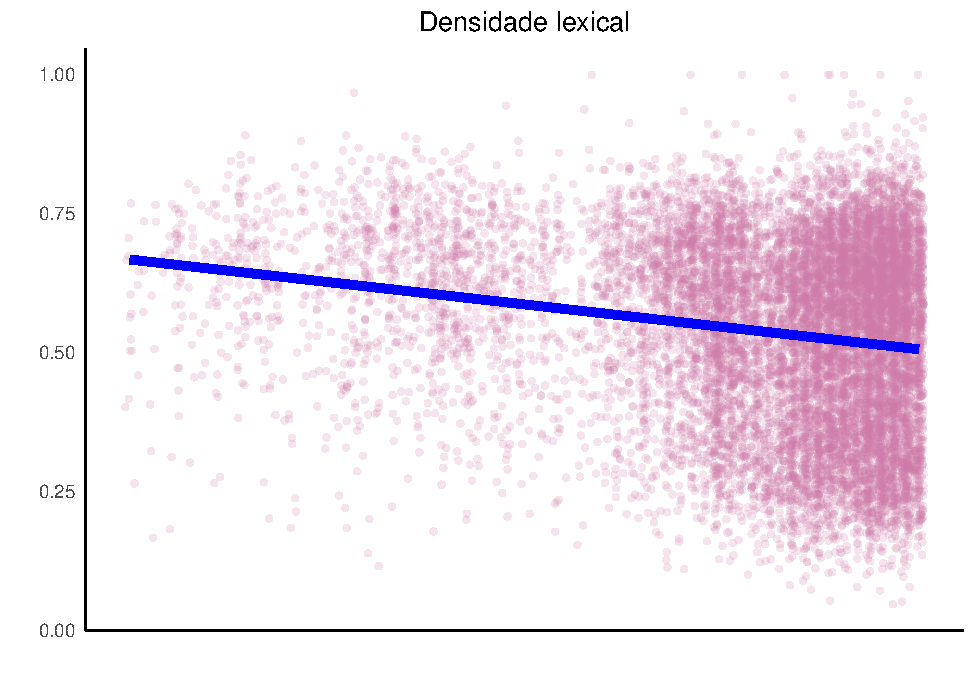
\includegraphics{avaliacaoLetrasDeForro_files/figure-latex/unnamed-chunk-9-1.pdf}

\begin{Shaded}
\begin{Highlighting}[]
\NormalTok{diversidadelexical_por_ano <-}\StringTok{ }\NormalTok{musicas }\OperatorTok
\StringTok{  }\KeywordTok{filter}\NormalTok{(decada }\OperatorTok{!=}\StringTok{ "NA"}\NormalTok{) }\OperatorTok
\StringTok{  }\KeywordTok{unnest_tokens}\NormalTok{(word, letra) }\OperatorTok
\StringTok{  }\KeywordTok{group_by}\NormalTok{(nome, ano) }\OperatorTok
\StringTok{  }\KeywordTok{summarise}\NormalTok{(}\DataTypeTok{lex_diversity =} \KeywordTok{n_distinct}\NormalTok{(word)) }\OperatorTok
\StringTok{  }\KeywordTok{arrange}\NormalTok{(}\KeywordTok{desc}\NormalTok{(lex_diversity)) }

\NormalTok{diversidadelexical_por_ano }\OperatorTok
\StringTok{  }\KeywordTok{ggplot}\NormalTok{(}\KeywordTok{aes}\NormalTok{(ano, lex_diversity)) }\OperatorTok{+}
\StringTok{    }\KeywordTok{geom_point}\NormalTok{(}\DataTypeTok{color =}\NormalTok{ colors[}\DecValTok{3}\NormalTok{],}
               \DataTypeTok{alpha =} \FloatTok{.2}\NormalTok{, }
               \DataTypeTok{size =} \DecValTok{2}\NormalTok{, }
               \DataTypeTok{position =} \StringTok{"jitter"}\NormalTok{) }\OperatorTok{+}\StringTok{ }
\StringTok{    }\KeywordTok{stat_smooth}\NormalTok{(}\DataTypeTok{color =} \StringTok{"black"}\NormalTok{, }\DataTypeTok{se =} \OtherTok{FALSE}\NormalTok{, }\DataTypeTok{method =} \StringTok{"lm"}\NormalTok{) }\OperatorTok{+}
\StringTok{    }\KeywordTok{geom_smooth}\NormalTok{(}\KeywordTok{aes}\NormalTok{(}\DataTypeTok{x =}\NormalTok{ ano, }\DataTypeTok{y =}\NormalTok{ lex_diversity), }\DataTypeTok{se =} \OtherTok{FALSE}\NormalTok{,}
                \DataTypeTok{color =} \StringTok{"blue"}\NormalTok{, }\DataTypeTok{lwd =} \DecValTok{2}\NormalTok{, }\DataTypeTok{method =} \StringTok{'gam'}\NormalTok{) }\OperatorTok{+}
\StringTok{    }\KeywordTok{ggtitle}\NormalTok{(}\StringTok{"Diversidade lexical"}\NormalTok{) }\OperatorTok{+}
\StringTok{    }\KeywordTok{xlab}\NormalTok{(}\StringTok{""}\NormalTok{) }\OperatorTok{+}\StringTok{ }
\StringTok{    }\KeywordTok{ylab}\NormalTok{(}\StringTok{""}\NormalTok{) }\OperatorTok{+}
\StringTok{    }\KeywordTok{scale_color_manual}\NormalTok{(}\DataTypeTok{values =}\NormalTok{ colors) }\OperatorTok{+}
\StringTok{    }\KeywordTok{theme_classic}\NormalTok{() }\OperatorTok{+}\StringTok{ }
\StringTok{    }\KeywordTok{theme_lyrics}\NormalTok{()}
\end{Highlighting}
\end{Shaded}

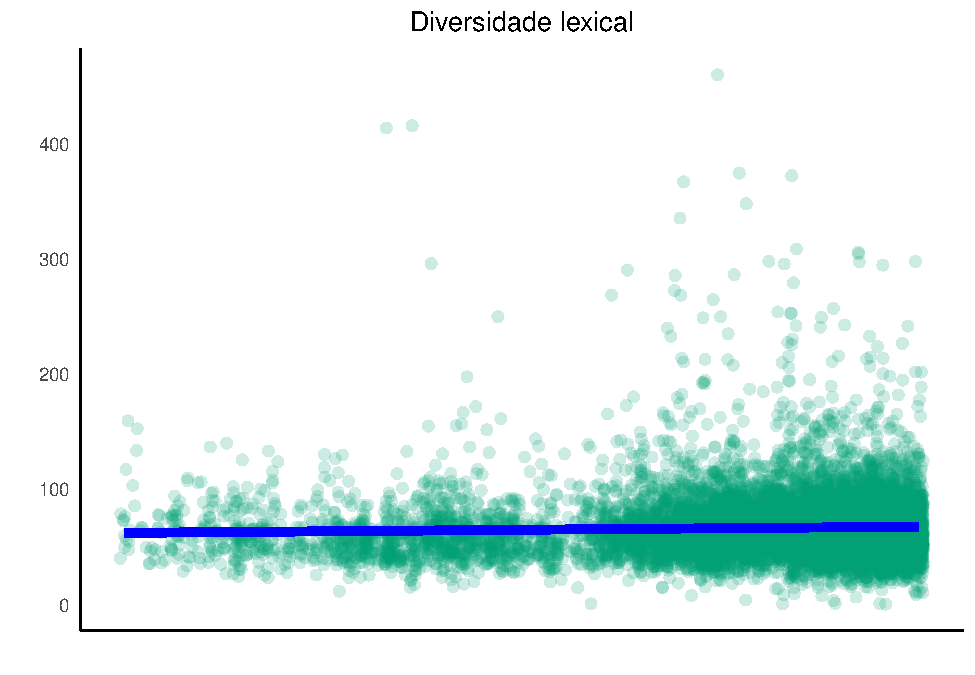
\includegraphics{avaliacaoLetrasDeForro_files/figure-latex/unnamed-chunk-9-2.pdf}

\hypertarget{frequencias-popularidade-de-palavras}{%
\section{Frequências / Popularidade de
palavras}\label{frequencias-popularidade-de-palavras}}

Visualização sobre a frequência com a qual as palavras mais aparecem por
letra em relação com o número de letras que mais contém cada uma dessas
palavras. Ou seja, a maior quantidade de palavras que aparecem em menos
letras do conjunto de dados.

TF: Frequência de palavras mais repetidas por letra DF: Frequência de
letras que contém cada palavra IDF: Frequência inversa por letra

A frequência é calculada por: TF - IFD = TF * IDF, onde FDI é a inversa
de DF 1 / DF

As palavras mais comuns devem ter o seu IDF e TF * IDF com o valor zero.

\begin{Shaded}
\begin{Highlighting}[]
\NormalTok{palavras_populares <-}\StringTok{ }\NormalTok{musicas }\OperatorTok
\StringTok{  }\KeywordTok{unnest_tokens}\NormalTok{(word, letra) }\OperatorTok
\StringTok{  }\KeywordTok{distinct}\NormalTok{() }\OperatorTok
\StringTok{  }\KeywordTok{filter}\NormalTok{(}\OperatorTok{!}\NormalTok{word }\OperatorTok\StringTok{ }\NormalTok{palavras_indesejadas) }\OperatorTok
\StringTok{  }\KeywordTok{filter}\NormalTok{(}\KeywordTok{nchar}\NormalTok{(word) }\OperatorTok{>}\StringTok{ }\DecValTok{3}\NormalTok{) }\OperatorTok
\StringTok{  }\KeywordTok{count}\NormalTok{(ano, word, }\DataTypeTok{sort =} \OtherTok{TRUE}\NormalTok{) }\OperatorTok
\StringTok{  }\KeywordTok{ungroup}\NormalTok{() }\OperatorTok
\StringTok{  }\KeywordTok{bind_tf_idf}\NormalTok{(word, ano, n)}

\KeywordTok{head}\NormalTok{(palavras_populares)}
\end{Highlighting}
\end{Shaded}

\hypertarget{visualizacao-enterior-com-graficos}{%
\section{Visualização enterior com
gráficos}\label{visualizacao-enterior-com-graficos}}

\begin{Shaded}
\begin{Highlighting}[]
\NormalTok{tf_idf_palavras_decadas <-}\StringTok{ }\NormalTok{musicas }\OperatorTok
\StringTok{  }\KeywordTok{unnest_tokens}\NormalTok{(word, letra) }\OperatorTok
\StringTok{  }\KeywordTok{distinct}\NormalTok{() }\OperatorTok
\StringTok{  }\KeywordTok{filter}\NormalTok{(}\OperatorTok{!}\NormalTok{word }\OperatorTok\StringTok{ }\NormalTok{palavras_indesejadas }\OperatorTok{&}\StringTok{ }\NormalTok{decada }\OperatorTok{!=}\StringTok{ 'NA'}\NormalTok{) }\OperatorTok
\StringTok{  }\KeywordTok{filter}\NormalTok{(}\KeywordTok{nchar}\NormalTok{(word) }\OperatorTok{>}\StringTok{ }\DecValTok{3}\NormalTok{) }\OperatorTok
\StringTok{  }\KeywordTok{count}\NormalTok{(decada, word, }\DataTypeTok{sort =} \OtherTok{TRUE}\NormalTok{) }\OperatorTok
\StringTok{  }\KeywordTok{ungroup}\NormalTok{() }\OperatorTok
\StringTok{  }\KeywordTok{bind_tf_idf}\NormalTok{(word, decada, n) }\OperatorTok
\StringTok{  }\KeywordTok{arrange}\NormalTok{(}\KeywordTok{desc}\NormalTok{(tf_idf))}

\NormalTok{top_tf_idf_palavras_decadas <-}\StringTok{ }\NormalTok{tf_idf_palavras_decadas }\OperatorTok\StringTok{ }
\StringTok{  }\KeywordTok{group_by}\NormalTok{(decada) }\OperatorTok\StringTok{ }
\StringTok{  }\KeywordTok{slice}\NormalTok{(}\KeywordTok{seq_len}\NormalTok{(}\DecValTok{8}\NormalTok{)) }\OperatorTok
\StringTok{  }\KeywordTok{ungroup}\NormalTok{() }\OperatorTok
\StringTok{  }\KeywordTok{arrange}\NormalTok{(decada, tf_idf) }\OperatorTok
\StringTok{  }\KeywordTok{mutate}\NormalTok{(}\DataTypeTok{row =} \KeywordTok{row_number}\NormalTok{())}

\NormalTok{top_tf_idf_palavras_decadas }\OperatorTok
\StringTok{  }\KeywordTok{ggplot}\NormalTok{(}\KeywordTok{aes}\NormalTok{(}\DataTypeTok{x =}\NormalTok{ row, tf_idf, }\DataTypeTok{fill =}\NormalTok{ decada)) }\OperatorTok{+}
\StringTok{    }\KeywordTok{geom_col}\NormalTok{(}\DataTypeTok{show.legend =} \OtherTok{NULL}\NormalTok{) }\OperatorTok{+}
\StringTok{    }\KeywordTok{labs}\NormalTok{(}\DataTypeTok{x =} \OtherTok{NULL}\NormalTok{, }\DataTypeTok{y =} \StringTok{"TF-IDF"}\NormalTok{) }\OperatorTok{+}\StringTok{ }
\StringTok{    }\KeywordTok{ggtitle}\NormalTok{(}\StringTok{"Palavras mais utilizadas com TF-IDF por decada"}\NormalTok{) }\OperatorTok{+}
\StringTok{    }\KeywordTok{theme_lyrics}\NormalTok{() }\OperatorTok{+}\StringTok{  }
\StringTok{    }\KeywordTok{facet_wrap}\NormalTok{(}\OperatorTok{~}\NormalTok{decada, }\DataTypeTok{ncol =} \DecValTok{3}\NormalTok{, }\DataTypeTok{nrow =} \DecValTok{3}\NormalTok{, }\DataTypeTok{scales =} \StringTok{"free"}\NormalTok{) }\OperatorTok{+}
\StringTok{    }\KeywordTok{scale_x_continuous}\NormalTok{( }\DataTypeTok{breaks =}\NormalTok{ top_tf_idf_palavras_decadas}\OperatorTok{$}\NormalTok{row, }\DataTypeTok{labels =}\NormalTok{ top_tf_idf_palavras_decadas}\OperatorTok{$}\NormalTok{word) }\OperatorTok{+}
\StringTok{    }\KeywordTok{coord_flip}\NormalTok{()}
\end{Highlighting}
\end{Shaded}

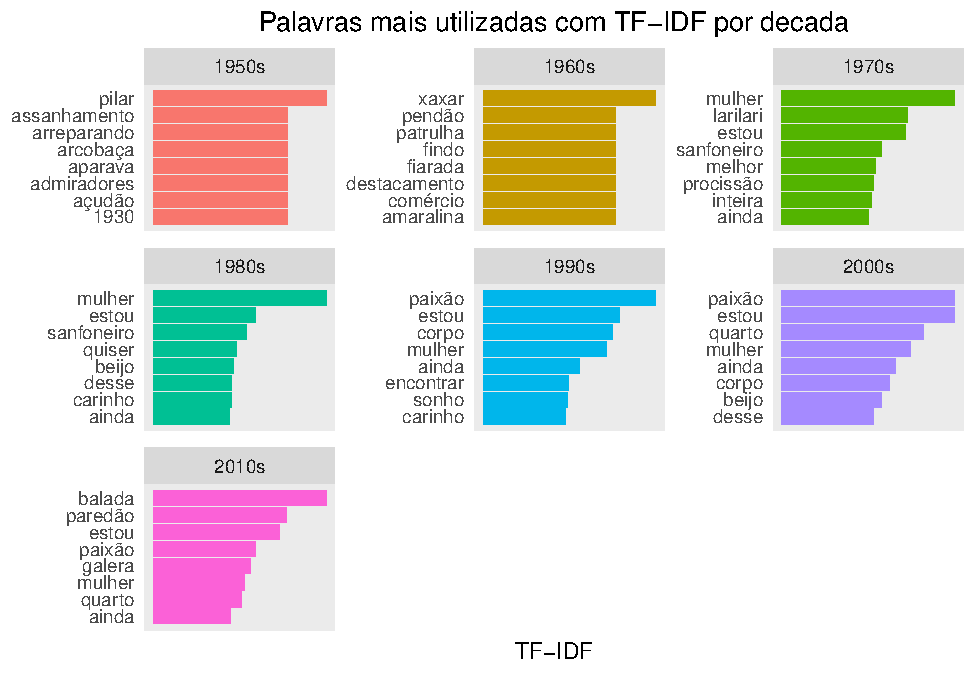
\includegraphics{avaliacaoLetrasDeForro_files/figure-latex/unnamed-chunk-11-1.pdf}

\hypertarget{nuvem-de-palavras-por-tf-idf}{%
\section{Núvem de palavras por
TF-IDF}\label{nuvem-de-palavras-por-tf-idf}}

\begin{Shaded}
\begin{Highlighting}[]
\NormalTok{wc <-}\StringTok{ }\NormalTok{tf_idf_palavras_decadas }\OperatorTok
\StringTok{  }\KeywordTok{arrange}\NormalTok{(}\KeywordTok{desc}\NormalTok{(tf_idf)) }\OperatorTok
\StringTok{  }\KeywordTok{select}\NormalTok{(word, tf_idf)}

\KeywordTok{wordcloud2}\NormalTok{(wc[}\DecValTok{1}\OperatorTok{:}\DecValTok{200}\NormalTok{, ], }
           \DataTypeTok{color =} \StringTok{"random-dark"}\NormalTok{,}
           \DataTypeTok{minSize =} \FloatTok{.05}\NormalTok{, }
           \DataTypeTok{ellipticity =} \FloatTok{.6}\NormalTok{, }
           \DataTypeTok{rotateRatio =} \DecValTok{1}\NormalTok{, }
           \DataTypeTok{size =} \FloatTok{.1}\NormalTok{, }
           \DataTypeTok{fontWeight =} \StringTok{"bold"}\NormalTok{, }
           \DataTypeTok{gridSize =} \DecValTok{1}\NormalTok{ )}
\end{Highlighting}
\end{Shaded}

\includegraphics{avaliacaoLetrasDeForro_files/figure-latex/unnamed-chunk-12-1.pdf}

\hypertarget{analise-de-sentimento}{%
\section{Analise de sentimento }\label{analise-de-sentimento}}

\hypertarget{discussao}{%
\section{Discussão}\label{discussao}}

Analizar de maneira ``macro'' o conjunto de dados, possibilitou avaliar
como as letras evoluíram no decorrer do tempo em termos de suas letras,
utilizando apenas processamento de texto natural. Considerando que a
análise relacionada ao significado dessas mudanças no decorrer do tempo
sejam subjetivas, por serem associadas a mudanças culturais, podemos
avaliar a maneira como as letras se modificaram e como as palavras foram
utilizadas nas décadas passadas nas letras de músicas do forró.

\ldots{}


\end{document}
